\documentclass[11pt,a4paper]{article}
% \usepackage{natbib}

\usepackage[utf8]{inputenc}

%\usepackage[margin=7cm]{geometry}
% \usepackage{listings}
% \usepackage{adjustbox}
% \usepackage{xcolor}
% \usepackage{verbatim}
% \usepackage{graphicx}%images
% \usepackage{fancyhdr}%for headers and footers
% \usepackage{adjustbox}
% \usepackage{verbatim}
% \usepackage{listings}
% \usepackage{fancyhdr}
% \usepackage{multirow}
% \usepackage{amsmath}
% \usepackage{mathtools}

% \usepackage{array}
% \usepackage{subcaption}
% \usepackage{float}
% \usepackage{csvsimple}
% \usepackage{filecontents}
% \usepackage{lscape}
% \usepackage{afterpage}
% \usepackage{hyperref}
% \usepackage{inconsolata}
% \usepackage{color}

\usepackage{mathpazo}
\usepackage{amsmath,amsfonts,amssymb,amsthm}
\usepackage{mathtools}
\usepackage{todonotes}


\usepackage{tikz}
\usetikzlibrary{arrows, automata, positioning}

% \usepackage{draftwatermark}
% \SetWatermarkText{Draft}
% \SetWatermarkScale{2}

% Math function

\DeclarePairedDelimiter{\ceil}{\lceil}{\rceil}
\DeclarePairedDelimiter{\floor}{\lfloor}{\rfloor}
\DeclarePairedDelimiter{\tuple}{\langle}{\rangle}
\newcommand{\darrow}{\, \downarrow \!\!}
\newcommand{\uarrow}{\, \uparrow \!\!}

% Theorems styles

\theoremstyle{definition}
\newtheorem{proposition}{Proposition}[subsection]
\newtheorem{example}{Example}[subsection]

% \newenvironment{conditions}
%   {\par\vspace{\abovedisplayskip}\noindent\begin{tabular}
%   {>{$}l<{$} @{${}={}$} l}}
%   {\end{tabular}\par\vspace{\belowdisplayskip}}
%
%
%   \newenvironment{conditions_bis}
%   {\par\vspace{\abovedisplayskip}\noindent\begin{tabular}
%   {>{$}l<{$} @{${}\in{}$} l}}
%   {\end{tabular}\par\vspace{\belowdisplayskip}}
%
% \definecolor{pblue}{rgb}{0.13,0.13,1}
% \definecolor{pgreen}{rgb}{0,0.5,0}
% \definecolor{pred}{rgb}{0.9,0,0}
% \definecolor{pgrey}{rgb}{0.46,0.45,0.48}
%
% \lstset{language=Python,
%   showspaces=false,
%   numbers=left,
%   showtabs=false,
%   breaklines=true,
%   showstringspaces=false,
%   breakatwhitespace=true,
%   commentstyle=\color{pgreen},
%   keywordstyle=\color{pblue},
%   stringstyle=\color{pred},
%   basicstyle=\ttfamily,
%   moredelim=[il][\textcolor{pgrey}]{$ $},
%   moredelim=[is][\textcolor{pgrey}]{\%\%}{\%\%}
% }
%
%
%
% \hypersetup{
%     colorlinks,
%     citecolor=black,
%     filecolor=black,
%     linkcolor=black,
%     urlcolor=black
% }
%
%
% % ------ HEADERS AND FOOTERS -----------
% % \lhead{INFO-F403}
% % \rhead{Project Report - Part 1}
% %\pagestyle{fancy}
% % \rfoot{\thepage}
% %\cfoot{}
% %\lfoot{Academic Year 2017-18}
%
\newcommand{\HRule}{\rule{\linewidth}{0.2mm}} %newcommand for cover page


\begin{document}

\begin{titlepage}

\begin{center}


\textsc{\LARGE universit\'e libre de bruxelles}\\[1.0cm]
\textsc{\Large D\'epartment d'Informatique}\\[1.0cm]

% Upper part of the page. The '~' is needed because \\
% only works if a paragraph has started.
\includegraphics[width=0.3\textwidth]{images/ulblogo.jpg}~\\[1cm]

\textsc{
\large MEMO-F-403 \\
\Large  Preparatory work for the master thesis
 \\[1.0cm]}
% Title
\HRule \\[0.3cm]

{ \huge \bfseries Data structures for \\
Partially Ordered Sets \\[0.3cm] }

\HRule \\[1cm]

% Author and supervisor
\noindent
\begin{center} \large

%\emph{Author:}\\
\Large Hakim \textsc{Boulahya}\\
\end{center}
\begin{center} \large

\emph{Supervised by} \\
\Large Emmanuel \textsc{Filiot} \\
\Large Guillermo A. \textsc{Pérez} \\[1cm]

\end{center}

% Bottom of the page
{\large \today}

\end{center}
\end{titlepage}


% \title{Implementing data structures for \\ Partially Ordered Set}
% \author{Hakim Boulahya}
%


% \maketitle

\newpage

\tableofcontents

\newpage

% \listoftodos

\newpage

\section{Introduction}

\subsection{Theoritical context}

Data structures play an important role in algorithms complexity.
With the objective to improve standard algorithms in automata theory,
researchers at ULB
have implemented new algorithms to solve
important problems therein.

\paragraph{}

One computer science
field that benefits from
those new implementation is formal verification of computer systems.
Verifiying a system consists in checking for a given model, if
it respect some formal specifications.
The major issue regarding problems
such as model checking is the state-space explostion problem.
Verification techiques are based on representing
models and specifications using automata, and the combination
can lead to an exponential blow-up. To face the state explosion
problem, methods that allow to represent larger system using
smaller models were developped. A known method is called
symbolic model checking and sometimes uses a data structure called
Binary Decision Diagram, used to represent boolean functions.

\paragraph{}

Another well known problem in verification is the synthesis problem.
It is, for
some model of a controller and an environment,
to check if there exists a winning strategy for the controller.
In order to develop more efficient algorithms to resolve such
problems Filiot et al. proposed in \cite{ltl_rea} a new approach
using antichains.
This is possible due to a partial order that exists on the state
space of the subset constructions. Since it has been
proven that the set is closed for this partial order,
antichains are well suited to resolve such problem.
Indeed, antichains are a set of incomparable elements, and
allow to represent partially ordered set in a more compact way.
This is possible through different operations on the antichains.
When the set of a partial order is closed, the antichains
can represent a bigger set by only keeping
either maximal or minimal elements,
and other elements can be retrieved using an upper or lower closure,
that is all the elements that are either bigger or smaller
compared to the elements of the antichains.
We define formally
those notions in section \ref{data_structures}.

\paragraph{}

The goal of this preparatory work is to motivate the interest that
are made in data structures for partially ordered sets,
especially antichains,
and why we need efficient
implementations.
It also defines the objectives
and recalls the state of the art of the various existing implementations.
In this work, we will mainly focus
on the usage of partially ordered sets and antichains in
automata theory-related problems.

\subsection{An application: language universality}

An example that highlights the use of antichains in automata theory is
the universality problem.
It is the problem that for a finite automaton, we want to
check if the language of this automaton equivalent to the language
of all the words on the alphabet. The universality problem is a classical
theoritical problem, and many verification-related problems can be
reduced to it.

\paragraph{}

Let $A = \tuple{Q_A, \Sigma, q_0, \delta, F_A}$ be a finite automaton,
we want to check whether
the language of $A$ is universal, that is, $L(A) = \Sigma^*$.
The language of $A$ is universal if and only if the language
of the complement of $A$ accepts no words, that is,
$L(A) = \Sigma^*$ if and only if $L(\bar{A}) = \emptyset$.
Therefore, the goal is to find a computation path of the
automaton on a word such that the path start in the initial state,
and the final target is a non-accepting state.

\paragraph{}

Let's first define an interesting proprety of non-deterministic automata
before explaining the use of antichains for the universality problem.
Let $q$ and $f$ be two subsets of states such that $q, f \subseteq Q_A$.
When reading a letter $\sigma$ on the deterministic equivalent
$A_d$, that is $q \xrightarrow{\sigma} f$, it is known that
for all sets of states $q' \subseteq q$, the resulting subset
$f'$, when computed on $A_d$ such that $q' \xrightarrow{\sigma} f'$,
it holds that $f' \subseteq f$.
%\todo{Does this proprety have a specific name ?}

\subsubsection{Concrete example}

\paragraph{}

Let's take the example from \cite{AC_universality}
shown in Figure \ref{fig:univnondet}. This example is a
non-deterministic finite automata with 4 states where
only the last state is non-accepting.
The goal is to check
if whether or not this automaton is universal.
One approach to check universality, is to check if the
complementary automaton accepts the empty set.
This is actually the standard algorithm that first builds
the equivalent deterministric automaton, builds the complement
and then check the emptiness of this final construction.
The complexity here rely on building the equivalent deterministic
which is exponential in size. The idea of the antichain based
algorithm is instead of determinize the automaton, to
do it implicitly by checking only maximal subsets of states.

\paragraph{}

Figure \ref{fig:univdet} shows the equivalent deterministic finite
automaton of the one
shown in Figure \ref{fig:univnondet}.
In the specific example of \ref{fig:univdet}, instead on checking
each state of the deterministic finite automaton, it is
better to check only the maximal path.
We refer to maximal path, a path where each subset of states
when computing any letter is maximal.


Indeed, the focus
is made on checking if the final state of a word computation is
non-accepting that is $q \xrightarrow{w} f$ we have that
 $f \cap F_A = \emptyset$.
Because of the
proprety of state inclusion, checking only the
maximal set of states is sufficient. Let $k=3$, computing the word $1^k$,
will lead to a maximal path for this automaton.
For any word $w < 1^k$
of size $k$ such that $w = \sigma_1..\sigma_k$ with $\sigma_i \in \Sigma$,
the path of computation will be included in the path of $1^k$,
\textit{i.e.} the subset of states $q_i$ will be included
in $p_i$, that is $q_i \subseteq p_i$,
corresponding respectively to the subsets of states
when reading the $i^{th}$ letter of the word $w$ and $1^k$.
Since the objective is to find the final state as a non-accepting,
if the final state is non-accepting for $1^k$,
that is $p_k \cap F = \emptyset$ then for the word $w$,
since $q_k \subseteq p_k$, it holds that $q_k \cap F = \emptyset$.
This method allow to bypass some computation, \textit{i.e.}
checking the intersection with the accepting states set, by only checking
the maximal subsets of states.


\begin{figure}
    \center
    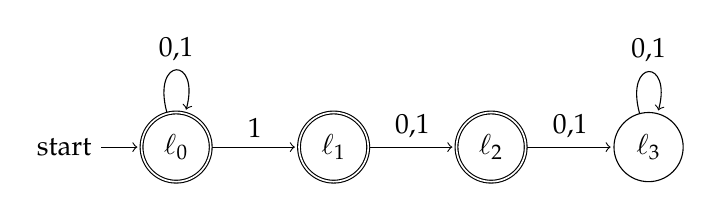
\begin{tikzpicture}[shorten >=1pt,node distance=2cm,on grid,auto]
       \node[state,accepting,initial] (l0)   {$\ell_0$};
       \node[state,accepting] (l1) [right=of l0] {$\ell_1$};
       \node[state,accepting] (l2) [right=of l1] {$\ell_2$};
       \node[state] (l3) [right=of l2] {$\ell_3$};
       \path[->]
        (l0)
        edge  node {1} (l1)
        edge [loop above] node {0,1} ()
        (l1)
        edge node {0,1} (l2)
        (l2)
        edge node {0,1} (l3)
        (l3)
        edge [loop above] node {0,1} ()
        ;
    \end{tikzpicture}

    \caption{Non-deterministic finite automaton from the
    family of automata $A_k$,
    from \cite{AC_universality}, with $k=3$.}
    \label{fig:univnondet}


\end{figure}

\begin{figure}
\center
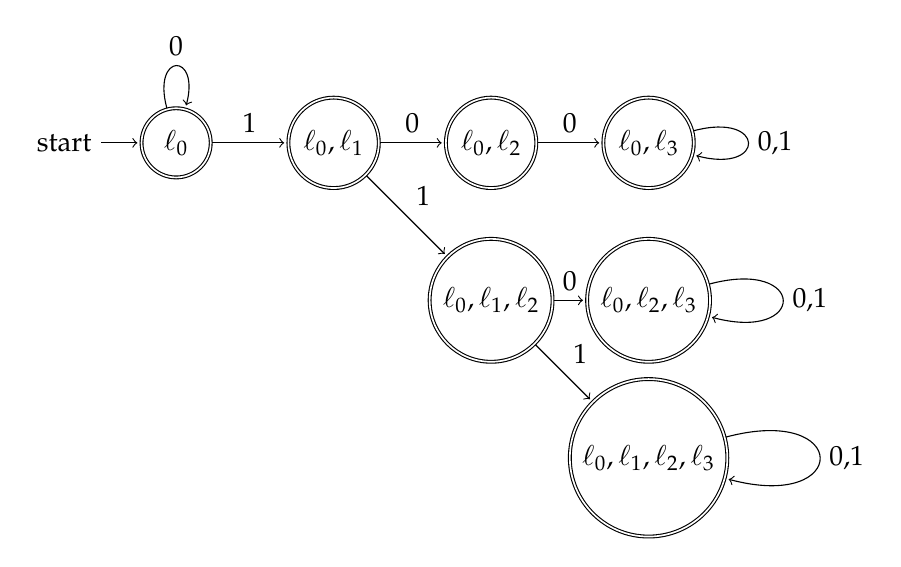
\begin{tikzpicture}[shorten >=1pt,node distance=2cm,on grid,auto]
   \node[state,accepting,initial] (l0)   {$\ell_0$};
   \node[state,accepting] (l0l1) [right=of l0] {$\ell_0,\ell_1$};
   \node[state,accepting] (l0l2) [right=of l0l1] {$\ell_0, \ell_2$};
   \node[state,accepting] (l0l1l2) [below=of l0l2] {$\ell_0,\ell_1,\ell_2$};
   \node[state,accepting] (l0l3) [right=of l0l2] {$\ell_0, \ell_3$};
   \node[state,accepting] (l0l2l3) [below=of l0l3] {$\ell_0,\ell_2,\ell_3$};
   \node[state,accepting] (l0l1l2l3) [below =of l0l2l3]
                                     {$\ell_0,\ell_1,\ell_2,\ell_3$};
   \path[->]
    (l0)
    edge  node {1} (l0l1)
    edge [loop above] node {0} ()
    (l0l1)
    edge node {0} (l0l2)
    edge node {1} (l0l1l2)
    (l0l2)
    edge node {0} (l0l3)
    (l0l1l2)
    edge node {0} (l0l2l3)
    edge node {1} (l0l1l2l3)
    (l0l3)
    edge [loop right] node {0,1} ()
    (l0l2l3)
    edge [loop right] node {0,1} ()
    (l0l1l2l3)
    edge [loop right] node {0,1} ()

    %       edge  node [swap] {1} (q_2)
    % (q_1) edge  node  {1} (q_3)
    %       edge [loop above] node {0} ()
    % (q_2) edge  node [swap] {0} (q_3)
    %       edge [loop below] node {1} ()
    ;
\end{tikzpicture}

\caption{Deterministic automaton equivalent of the non-deterministic
automaton shown in Figure \ref{fig:univnondet}.}
\label{fig:univdet}

\end{figure}


% The only way to compute the complementary of $A$ is to first
% determinise it, which is hard. Let define $A_d$ as the deterministic finite
% automaton (DFA) of $A$ such that $L(A_d) = L(A)$.
% When $A$ is transformed to $A_d$,
% the set of states of the DFA is the powerset of states,
% that is a state of the DFA $A_d$ is represented by a subset of state of $A$.
% Now if $L(\bar{A})$ is the empty set,
% it means that there is no set of states that for which there exists a word
% such that, when computed by $\bar{A}$,
% this word is accepted.
% With the set
% $X = \{ P,  \subseteq Q, P' \subseteq Q, P' \cap \bar{F} = \emptyset
% | \exists w \in \Sigma^* s.t. P \xrightarrow{w} P'\}$, it provides
% a way to check the existence such set of states.
% The goal is to show that if there exists
% no set of states $P'$ such that $P' \cap F = \emptyset$ i.e.
% $X = \emptyset$, then it is shown that $L(\bar{A}) = \emptyset$, therefore
% $A$ is universal. The difficulty of the problem arise at the computation
% of $X$. Checking intersection between the accepting states set and all
% the subsets is costly.
% \todo{Costly vs expensive vs complexe vs hard etc..}
% For a subset $P \subseteq Q$, for all subsets $p$ such that $p \subseteq P$,
% it is known that, computing the word $w$ starting from $p$ or $P$, will lead
% to the same final state. Therefore it is more interesting to compute
% the maximal sets $\ceil{X}$, which correspond to an antichain of set of
% states that are $\subseteq$-incomparable. In section \ref{data_structures},
% we give formal definition of notions such as maximal sets or incomparable
% elements.
% \todo{Include Xi explanation}


\paragraph{}

The algorithm proposed in \cite{AC_universality}, doesn't build
the deterministic automaton, but rather does it implicitly.
It builds iteratively a set of subsets of states
that have as initial targets the non-accepting states.
At each iteration,
it adds direct
predecessors to the targets, until a fixed point is reached.
Also, at each iteration,
only maximal set of states, that is an antichain,
based on the inclusion partial order are kept
in memory for the next iteration.
The final condition is to check if the initial state is found
in the targets. It the initial state is included, it means that
there exists a word such that it is not accepted by
the automaton, it means that the automaton is not universal.


% In
% \cite{AC_universality}, the algorithm proposed follow an equivalent
% idea by using game theory. The universality problem is reduce to
% a two-player reachability game, which can be done in polynomial time.
% The objective of the game is for the protagonist to establish that
% the automaton $A$ is not universal. To this end, the protagonist will
% provide a word, a letter at a time, and find a strategy that try
% to show that $A$ ends in a rejecting state.
% The protagonist only has a strategy to win the game if and only if $A$ is
% not universal.

\subsection{Objective}

The objective of the final work
is to provide an efficient implementation of different
data structures that allow to compactly
represent partially ordered sets, specifically antichains.
The first step is to implement in Java, classes that will be provided to
the \texttt{Owl} library \cite{owl}.
\texttt{Owl} is a LTL to deterministic automata translations tool-set written
in \texttt{Java}. We present in more details
the \texttt{Owl} library in section \ref{sec:owl}.
A second step will be to implement
antichain-based algorithms using the new antichains implementation and
study the performance.
%\todo{Include examples from Guillermo correction}

\subsection{Related work}

There are two interesting implementations that were found.
The first one is \texttt{AaPAL} (
Antichain and Pseudo-Antichain Library), a generic
library that was implemented in the frame of
Aaron Bohy's PhD thesis \cite{bohy_phd}
to provide an antichain library. It is implemented in \texttt{C}.
The other implementation of antichains
have been done
by De Causmaecker and De Wannemacker in \cite{causemaecker1}. The algorithms
to find the ninth Dedekind number uses antichains and they needed to
implement a representation of antichains. Their implementation is using
\texttt{Java}.
To improve efficiency and performances, Hoedt in \cite{hoedt} has extended
\cite{causemaecker1} antichains implementation by using bit sequence
instead of tree reprensentation.

\subsection{Structure of the preparatory work}

This paper is the introduction to next year thesis, therefore
the content concern only the preliminaries. The goal is to
properly define the subject,
existing implementations and the desired objectives.
In section \ref{data_structures}, we formally define antichains,
and give examples of such data structures. In section \ref{impl},
we summarize the work that has been done by others
for antichains implementation. In section \ref{conclusion}, we propose
an overview of next year work and possibilities.

\newpage

\section{Data Structures}

\label{data_structures}

\paragraph{}

In this section, we will provide formal definitions of the data
structures that we will implement. We recall the notion of binary relations
and important propreties of such relations.
We then define partially ordered set, totally order set and closed set.
Finally we give a formal definition for antichains.

\paragraph{}

The definitions and examples for this section are based on \cite{bohy_phd}
and \cite{maquet_phd}.


\subsection{Binary relations}

\paragraph{}

A binary relation for an arbitrary set $S$ is
a set of pair $R \subseteq S \times S$.
There are five important properties: reflexitivity, transitivity,
symmetry, antisymmetry and total.

\paragraph{}

A relation $R$ on $S$ is said to be:

\begin{itemize}
    \item Reflexive:
    iff $\forall s \in S$ it holds that $(s, s) \in R$
    \item Transitive:
    iff $\forall s_1, s_2, s_3 \in S$,
    if ($s_1, s_2) \in R$ and $(s_2, s_3) \in R$
    then it holds that $(s_1, s_3) \in R$
    \item Symmetric: iff $(s_1, s_2) \in R$ then $(s_2, s_1) \in R$.
    \item Antisymmetric: iff $(s_1, s_2) \in R$
    and $(s_2, s_1) \in R$ then $s_1 = s_2$
    \item Total: iff $\forall s_1, s_2 \in S$ then $(s_1, s_2) \in R$
    or $(s_2, s_1) \in R$

\end{itemize}

\paragraph{Orders}

A \textit{partial order} is a binary relation that is \textit{reflexive},
\textit{transitive} and \textit{antisymmetric}. We note a
partial order relation by $R$.
We note $s_1 R  s_2$ to show the belonging of
a binary relation to a partial order, which is equivalent
to $(s_1, s_2) \in \ R$.
A \textit{total order} is a partial order that is \textit{total}.

\begin{example}

For example, the comparison of natural numbers is a partial order.
Let $\leq$ be a binary relation on $\mathbb{N}$
such that $\leq \ \subseteq \mathbb{N}^2$. The binary relation is defined
following the usual semantic of the symbol, i.e. $n_1 \leq n_2$ if and
only if $n_1$ is smaller or equal to $n_2$.
Based on this, $\leq$ is a partial order. It is
reflexive, transitive and antisymmetric.
The binary relation $\leq$ on natural numbers is actually a total
order since all the natural numbers can be compared against each other.

\end{example}

\subsection{Partially ordered set}

\paragraph{}

An arbitrary set $S$ associated with a partial order $\preceq$
is called a \textit{partially ordered set} or \textit{poset}.
It is denoted by the pair $\langle S, \preceq \rangle$.

\paragraph{Comparable}

Let $s_1, s_2 \in S$ and $\tuple{S, \preceq}$ a poset.
The two elementes $s_1$ and $s_2$ are said to be \textit{comparable} if either
$s_1 \preceq s_2$ or $s_2 \preceq s_1$. If neither of those two comparisons
are correct, then $s_1$ and $s_2$ are said to be \textit{incomparable}.


\paragraph{Bounds} Let $\tuple{S, \preceq}$ a partially ordered set.
A \textit{lower bound} of $P \subseteq S$ is an element $s \in S$
such that for all $p \in P$, it holds that $s \preceq p$.
The \textit{greatest lower bound} of elements of a set $P \subseteq S$
is an element $s \in S$ defineds as follow:
for all $p \in P$
it holds that $s \preceq p$, and for all $s' \in S$ we have that
if $s' \preceq p$ then $s' \preceq s$.

The greatest lower bound is unique. It means that if two elements
$s_1, s_2 \in S$ are $\preceq$-incomparable and for a subset $P \subseteq S$,
for all $p \in P$, if it holds that $s_1 \preceq p$ and $s_2 \preceq p$
and if all others elements $s' \in S$ with $s'$ a lower-bound
for $P$ such that $s' \preceq s_1$ and $s' \preceq s_2$;
the greatest lower bound is said to be undefined.

For a set of two elements
$P = \{p_1, p_2\}$, we denote by $p_1 \sqcap p_2$ the greatest lower bound.

\paragraph{Lattices} A \textit{lower semilattice} is a poset
$\tuple{S, \preceq}$ where for all pair of elements $s_1, s_2 \in S$,
we have that the greatest lower bound $s_1 \sqcap s_2$ exists.


%\todo{Include definition of least upper bound, if necessary}

\begin{example}
    % the inclusion $\subseteq$ is a partial order on
    % $2^{\mathbb{N}}$,
    % the power set of natural numbers.

    \label{eg:poset2}

%A more interesting example is the set inclusion comparison.
%Let $A$ be automaton defined in Example \ref{universality_eg}.
Let $\tuple{2^{Q_A}, \subseteq}$, a poset with
$Q_A$ a set of 3 elements. Figure \ref{fig:eg_antichain1}
shows a graph with the incomparable elements of such poset.

\begin{figure}

    \center
    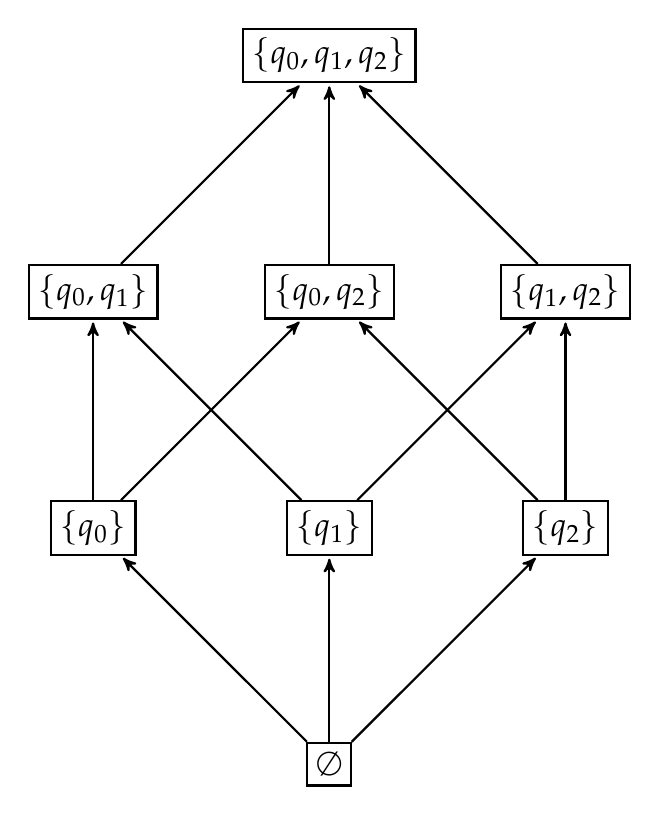
\begin{tikzpicture}[->,>=stealth',shorten >=1pt,auto,node distance=3cm,
                    thick,
                    main node/.style=
                    {rectangle,draw,font=\sffamily\large\bfseries}]

  \node[main node] (012) {$\{q_0, q_1, q_2\}$};
  \node[main node] (02) [below of=012] {$\{q_0, q_2\}$};
  \node[main node] (01) [left of=02] {$\{q_0, q_1\}$};
  \node[main node] (12) [right of=02] {$\{q_1, q_2\}$};
  \node[main node] (1) [below of=02] {$\{q_1\}$};
  \node[main node] (0) [left of=1] {$\{q_0\}$};
  \node[main node] (2) [right of=1] {$\{q_2\}$};
  \node[main node] (EMPTY) [below of=1] {$\emptyset$};

  \path[every node/.style={font=\sffamily\small}]
      (02) edge node [] {} (012)
      (01) edge node [] {} (012)
      (12) edge node [] {} (012)

      (0) edge node [] {} (01)
          edge node [] {} (02)
      (1) edge node [] {} (01)
          edge node [] {} (12)
      (2) edge node [] {} (02)
          edge node [] {} (12)

      (EMPTY) edge node [] {} (0)
              edge node [] {} (1)
              edge node [] {} (2)
    ;
\end{tikzpicture}
    % \begin{tikzpicture}[->,>=stealth',shorten >=0.5pt,auto,node distance=2.3cm,
    %                     thick,
    %                     main node/.style=
    %                     {rectangle,draw,font=\sffamily\large\bfseries}]
    %
    %   % \node[main node] (012) {$\{q_0, q_1, q_2\}$};
    %   \node[main node] (0)  {$\{q_0\}$};
    %   \node[main node] (1) [right of=0] {$\{q_1\}$};
    %   \node[main node] (2) [right of=1] {$\{q_2\}$};
    %   \node[main node] (3) [right of=2] {$\{q_3\}$};
    %
    %   \node[main node] (01) [above of=0] {$\{q_0, q_1\}$};
    %   \node[main node] (02) [right of=01] {$\{q_0, q_2\}$};
    %   \node[main node] (03) [right of=02] {$\{q_0, q_3\}$};
    %   \node[main node] (12) [right of=03] {$\{q_1, q_2\}$};
    %   \node[main node] (13) [right of=12] {$\{q_1, q_3\}$};
    %   \node[main node] (23) [right of=13] {$\{q_2, q_3\}$};
    %
    %   \node[main node] (012) [above of=01] {$\{q_0, q_1, q_2\}$};
    %   \node[main node] (013) [right of=012] {$\{q_0, q_1, q_3\}$};
    %   \node[main node] (123) [right of=013] {$\{q_1, q_2, q_3\}$};
    %   \node[main node] (023) [right of=123] {$\{q_0, q_2, q_3\}$};
    %
    %   \node[main node] (0123) [above of=123] {$\{q_0, q_1, q_2, q_3\}$};
    %
    %   \node[main node] (EMPTY) [below of=1] {$\emptyset$};
    %
    %   \path[every node/.style={font=\sffamily\small}]
    %       % (01) edge node [] {} (012)
    %       % (02) edge node [] {} (012)
    %       % (03) edge node [] {} (012)
    %       % (12) edge node [] {} (012)
    %       % (13) edge node [] {} (012)
    %       % (23) edge node [] {} (012)
    %       %
    %       (0)   edge node [] {} (01)
    %             edge node [] {} (02)
    %             edge node [] {} (03)
    %       (1) edge node [] {} (01)
    %           edge node [] {} (12)
    %           edge node [] {} (13)
    %       (2)   edge node [] {} (02)
    %             edge node [] {} (12)
    %             edge node [] {} (23)
    %       (3) edge node [] {} (03)
    %             edge node [] {} (13)
    %             edge node [] {} (23)
    %       %
    %       (EMPTY) edge node [] {} (0)
    %               edge node [] {} (1)
    %               edge node [] {} (2)
    %               edge node [] {} (3)
    %     ;
    % \end{tikzpicture}
    \caption{Example of antichains using
    the poset $\tuple{2^{Q_A}, \subseteq}$,
    with $Q_A$ the set of states of an automaton $A$, which correspond
    to $Q_A = \{q_0, q_1, q_2\}$. Each directed edge of the graph
    correspond to a valid comparison using the set inclusion $\subseteq$.
    For example
    $\{q_0\} \rightarrow \{q_0, q_1\}$ corresponds to
     the inclusion $\{q_0\} \subseteq \{q_0, q_1\}$. Two elements of the graph
     with no connection, means that the elements are incomparable. For
     example, $\alpha = \{\{q_0\}, \{q_1\}, \{q_2\}\}$ is a set
     of incomparable elements and $\alpha$ is called an antichain.}
     \label{fig:eg_antichain1}
\end{figure}

\end{example}

\subsection{Antichains}

\paragraph{Closed sets}

A closed set is a set $L \subseteq S$
of a lower semilattice $\langle S, \preceq \rangle$
where $\forall \ell \in L$ we have that $\forall s \in S$ such that
$s \preceq \ell$, then $s \in L$.
Note that for two closed sets $L_1, L_2 \subseteq S$, we have that
$L_1 \cup L_2$ and $L_1 \cap L_2$ are also closed sets,
but $L_1 \setminus L_2$ does not result necessarily to a closed set.

\paragraph{Maximal/minimal elements} We denote by $\ceil{L}$
the set of maximal elements of a closed set $L$ which
%\todo{Meaning of | vs . vs : in set definition ?}
correspond to $\ceil{L} =
\{ \ell \in L | \forall \ell' \in L : \ell \preceq \ell'
 \Rightarrow \ell = \ell' \}$. Alternatively, to represent the set of minimal
 elements, the noation $\floor{L}$ is used which has the following semantic
$\floor{L} = \{ \ell \in L | \forall \ell' \in L :  \ell' \preceq \ell
 \Rightarrow \ell = \ell' \}$.


\paragraph{Closure} A \textit{lower closure} of a set $L$ on $S$
noted $\darrow L$ is the set of all elements of $S$ that are
\textit{smaller or equal} to an element of $L$ i.e.
$\darrow L = \{ s \in S \ | \ \exists \ell \in L \cdot s \preceq \ell\}$.
Note that for a closed set $L$ we have that $\darrow L = L$.

\paragraph{Antichain}

An \textit{antichain} of a poset $\tuple{S, \preceq}$
is a set $\alpha \subseteq S$ where all element of $\alpha$
are incomparable with respect to the partial order $\preceq$.
Otherwise, if all elements are comparable the set is called a \textit{chain}.
Antichains allow to represent closed set in a more compact way.
For a closed set $L \subseteq S$ we can retrieve all elements of $L$ by using
the antichain $\alpha = \ceil{L}$. With respect
to the definition of the lower closure we have that $\darrow \alpha = L$.

\subsection{Operations on antichains}

\paragraph{}

This section list the classical propreties of antichains.
All the examples are based on the poset
defined in Example \ref{eg:poset2}.

\begin{proposition}

\label{antichains_ops}

Let $\alpha_1, \alpha_2 \subseteq S$ two antichains and $s \in S$:

\begin{itemize}
    \item $s \in \darrow \alpha_1$
    iff $\exists a \in \alpha_1$ such that $s \preceq a$

    \begin{example}
        Let $\alpha_1 = \{\{q_0, q_1\}\}$, $\{q_0\}$ belongs to
        the lower closure $\darrow{\alpha_1}$ because,
        $\{q_0\} \subseteq \{q_0, q_1\}$.
    \end{example}

    \item $\darrow \alpha_1 \subseteq \darrow \alpha_2$
    iff $\forall a_1 \in \alpha_1,
    \exists a_2 \in \alpha_2$ such that $a_1 \preceq a_2$
    \begin{example}
    Let $\alpha_1 = \{\{q_0\}, \{q_1\}\}$ and
    $\alpha_2 = \{\{q_0, q_1\}\}$,
    $\darrow{\alpha_1} \subseteq \darrow{\alpha_2}$, since
    all elements of $\alpha_1$ are included
    in the single element of $\alpha_2$.
    \end{example}
    \item $ \darrow \alpha_1 \ \cup \darrow \alpha_2 =
    \darrow \ceil{\alpha_1 \cup \alpha_2}$

    \item $\darrow \alpha_1 \ \cap \darrow \alpha_2 =
    \darrow \ceil{\alpha_1 \sqcap \alpha_2}$ where $\alpha_1 \sqcap \alpha_2$
    is defined as
    $\alpha_1 \sqcap \alpha_2 = \{a_1 \sqcap a_2 | a_1
    \in \alpha_1, a_2 \in \alpha_2\}$, that is the greatest lower bound
    of elements between the two antichains.

\end{itemize}

\end{proposition}



% \subsection{Pseudo-antichains}
%
% \paragraph{}
%
% An antichain is a subset of $S$ that allow to represent in a compact way
% a set $L \subseteq S$ that is not necessarily closed.

\newpage


\section{Existing implementations}

\label{impl}

In this section, we recall a state of the art of the different
antichain implementation. Two academic implementation were found.
First, we describe the \texttt{AaPAL}
library. Secondly, we describe another antichain utilization
in the context of the Dedekind problem.

\subsection{AaPAL}

Bohy's \textbf{A}ntichain
\textbf{a}nd \textbf{P}seudo-\textbf{A}ntichain \textbf{L}ibrary \cite{aapal}
is an open-source generic library for the manipulation
of antichains and pseudo-antichains data structures,
implemented in \texttt{C}. In this section we will mainly focus
on the implementation of antichains.
%\todo{Pseudo-antichains might be interesting for next year maybe ?}


\paragraph{Antichain representation}

An antichain is represented by a \texttt{struct}, containing as attributes
the size of the antichain, and the incomparable elements of the antichains,
as a list. The list is manipulated using the \texttt{GSList} object
from the \texttt{glib} library.
To allow modularity, the type of the elements
is \texttt{void}.
%\todo{Find usage of AaPAL (see Bohy's PHD)}

\paragraph{Operations}

The operations implemented in \texttt{AaPAL}
are the union, intersection and appartenance
defined in Proposition \ref{antichains_ops}.
An interesting remark is that most of the complexity is given as a paramater
to the functions. For example the function to compare two elements in
an antichain is given as a parameter. It means that the complexity to define
the domain of the antichain, must be implemented in the compare function.
Same pattern goes for the intersection operation,
the function to compute the intersection must be provided by the user.
Also basic
operations such as creating an antichain,
adding an element to
an antichain, checking emptiness or cloning an antichain are implemented.
in \texttt{AaPAL}.

\subsection{Antichains for Dedekind's problem}

\label{sota_hoedts}

\paragraph{Dedekind's problem}

The Dedekind's problem correspond to a problem introduced by Richard
Dedekind in the 19th century. He defined a rapidly growing sequence
of natural numbers. The $n_{th}$ Dedekind number is the count
of antichains in the powerset of set with $n$ elements.

\paragraph{}

De Causemaecker and De Wannemacker \cite{causemaecker1} improved and
implemented a multithreaded algorithm to find the $n^{th}$ Dedekind number
that allow to compute the $n^{th}$ Dedekind number from the powerset
of a set with $(n-2)$-elements, that is re-use the number of antichains
for $(n-2)$-set to compute the $n{th}$ Dedekind number.


\paragraph{}

De Causemaecker and De Wannemacker only provide the executable of
their algorithm in their paper for
the Dedekind algorithm \cite{causemaecker1}. Hoedt proposed in \cite{hoedt}
an algorithm to find the ninth Dedekind number, which requires a representation
of antichains. The representation used is an extension of the implementation
proposed by De Causmaecker and De Wannemacker. The source of his
implementation was found in is personal GitHub \cite{hoedt_src}.
We will therefore only focus on the implementation
of Hoedt, which is an extension of the implementation proposed
by De Causmaecker and De Wannemacker, but by representing an antichains
using bitarray-like methods.

\paragraph{Antichains representation}

According to Hoedt in
\cite{hoedt}, the first proposed representation
in \cite{causemaecker1} was done by using
a \texttt{TreeSet}. With the objective to improve the performance of
the important operations, for example the intersection, Hoedt used
another way to represent antichains, by using a bitarray-like representation.
The goal of the bitarray representation is to represent set of natural numbers
by a binary representation. For example the subset $\{1, 2\}$ would be
represented by the binary number $11_2$ and the subset $\{1, 3\}$
by $101_2$ corresping respectively to $3_{10}$ and $5_{10}$. Then an antichain
is represented by enabling the bit of the corresponding number of an element
of the antichain. Therefore, an antichain $\alpha = \{\{1, 2\}, \{1, 3\}\}$
is represented by the bitarray  where the bit at indices $3$ and $5$
are enabled, that is $10100$.

\newpage

\section{Next year overview}

\label{conclusion}

This paper introduces the preliminaries for the thesis
and gives a first insight of the final
work objectives. Therefore in this section, we will first describe
the \texttt{Owl} project, the library where our contribution should
be implemented. Finally we give a first possibility for the
antichain implementation.

\subsection{Owl library}

\label{sec:owl}

\paragraph{Description from the offical website \cite{owl}}
\textit{Owl (Omega Word and automata Library)
is a library and tool-set tailored for – but not
limited to – semantic-based translations
from LTL to deterministic automata.}

\paragraph{}

\texttt{Owl} is a library developed at the
\textit{Technische Universität München}
maintained by Salomon Sickert and the community.
The library can be used as a command line tools or from an
online version available at \textit{http://rabinizer-owl.pe.hu/}.
It is implemented in \texttt{Java}.
It provides automata transformation, such as LTL formulae
to Rabin automata, and analysis
tools as well as synthesis algorithms.
Symbolic antichain-based algorithms are missing, which motivate
our work to implement such algorithms and will provide
to the community an enriched library.



\subsection{Requirements}

\paragraph{}


Different requirements were defined regarding the desired implementation.
The first requirement is that the library will have to be used in
\texttt{Owl}, therefore the language of reference is \texttt{Java 10}.
the choice of the language, even if highly encouraged by
the library \texttt{Owl}, is also interesting due to features that
are available in \texttt{Java}. One of which would interest us
in our work, is the ability to profile our implementation.
Profiling is a form of measurement of the time complexity or
the memory usage of a program execution. There exists multiple
tools to profile a \texttt{Java} program such as VisualVM, YourKit
or JProfiler.

% \subsection{Summary of objectives}
%
% \paragraph{}
%
% The main focus of the thesis is to be able to provide an efficient
% implementation of antichains in \texttt{Java}.
% The first step is to provide an interface for the different operations that
% can be applied to antichains. We then give a description
% of the implementation.
% Antichains provide a way to represent
% in a compact way partially ordered set that are closed. Pseudo-antichains
% are an extension of antichains and provide a compact way to represent
% partially ordered sets. Pseudo-antichains does not specifically require
% closed set.
%
% Our goal is to find a way to not keep all the closure all
% element of the antichain in memory, but be able to retrieve those elements
% or check the belonging of a closure element from the incomparable elements
% of the antichain.


\subsection{Framework and implementation}

\paragraph{}

% The \texttt{Java}
% interface proposed in \ref{oset_git} gives a first overview
% of the desired implementation.

The goal will be to try to find a good
way to implement antichains representation
and operations. One of the possible way to do so is to provide
a framework that will allow to implement
operations functions
depending on the universe of the antichains.
In \texttt{AaPAL} all the complexity
is implemented in the \texttt{compare\_elements} that must be given
to the library functions. It that case, all the complexity
must be implemented by the user to define the universe of the antichains.
An example of specific implementation for natural numbers is the one
proposed by Hoedt, presented in section \ref{sota_hoedts},
using bitarray. A first step
is to proposed an framework for users to implement the specifics of the
universe necessary for their algorithms. Next year thesis objective will
be to propose a generic and abstract API, and implement specifics
for known universe and test them on state-of-the-art algorithms,
especially in automata theory.

%\todo{Include algorithms to test i.e. Boolean function from Guillermo}

\newpage

\bibliographystyle{alpha}
\bibliography{thesis}

\end{document}
